\documentclass[11pt]{article}

\usepackage[margin=1in]{geometry}
\usepackage{amsmath,amssymb}
\usepackage{booktabs}
\usepackage{graphicx}
\usepackage{hyperref}
\usepackage{enumitem}
\usepackage{float}

\title{Empirical Evaluation of ProtoHedge:\\Interpretable Deep Hedging with Real Market Data}
\author{Yanis Zaim \and \textit{Advisor: TODO}}
\date{\today}

\begin{document}
\maketitle

\begin{abstract}
ProtoHedge was introduced as an interpretable alternative to black-box deep hedging, with the original evidence centered on synthetic environments. This paper studies whether the same prototype-based idea remains competitive when trained and evaluated on historical option-hedging episodes. We construct a real-data hedging environment from WRDS-sourced equity and ETF option data, evaluate ProtoHedge across a 10-ticker panel, and compare it with unhedged exposure, rule-based delta baselines, and vanilla Deep Hedging under a common robust protocol. The main empirical result is favorable to the ProtoHedge thesis: a mean-oriented ProtoHedge frontier achieves the best average mean performance across the panel, while a tail-oriented ProtoHedge frontier achieves the best average CVaR$_{5\%}$, and both do so with lower position-bound occupancy than vanilla Deep Hedging. We also verify interpretability directly by examining prototype concentration, regime-dependent prototype usage, and nearest historical states associated with the dominant prototypes. A final planned extension to Asian options is included as a placeholder subsection, with results to be added after the last path-dependent run is complete.
\end{abstract}

\section{Methods}

\subsection{ProtoHedge for Empirical Deep Hedging}
The empirical question in this paper is not whether ProtoHedge should dominate every black-box hedge on every metric. The scientific question is whether a prototype bottleneck can preserve most of the hedging performance of a flexible neural policy while exposing a smaller and more interpretable decision structure.

Let $x_t$ denote the current market state and let $a_t$ denote the hedge action. In vanilla Deep Hedging, a neural network maps $x_t$ directly to $a_t$. In ProtoHedge, the state is first embedded into a representation $z_t = f_\theta(x_t)$ and compared with a dictionary of $K$ prototypes $\{p_k\}_{k=1}^K$. Similarity weights are then computed as
\[
\alpha_{t,k} = \frac{\exp\{-d(z_t,p_k)\}}{\sum_{j=1}^K \exp\{-d(z_t,p_j)\}},
\]
and the action is formed as a convex combination of prototype actions,
\[
a_t = \sum_{k=1}^K \alpha_{t,k} b_k,
\]
where $b_k$ is the learned action associated with prototype $k$. This is the same structural idea as in the original ProtoHedge paper: the hedge acts through a small set of representative states rather than through a fully unconstrained latent policy.

For the empirical experiments, prototypes are extracted from standardized training states using the same ProtoHedge-style offline procedure. We evaluate prototype counts $K \in \{10,25,50,100\}$, two prototype sources (states derived from a spot-delta rule and states derived from a trained vanilla Deep Hedging policy), and both weighted and unweighted similarity.

\subsection{Historical Episode Construction}
The real-data panel is built from WRDS-sourced U.S. options and underlying price data. We focus on call-option hedging episodes and construct a fixed-horizon at-the-money short-call liability for each episode. The underlying panel consists of 10 liquid markets:
\[
\text{AAPL},\ \text{IWM},\ \text{NVDA},\ \text{QQQ},\ \text{SPY},\ \text{TLT},\ \text{XLE},\ \text{XLF},\ \text{XLK},\ \text{XLV}.
\]
These cover broad-market ETFs, sector ETFs, a Treasury ETF, and large-cap single names. The cleaned sample spans January 11, 2005 through December 31, 2024.

For each underlying and date, we identify the nearest at-the-money call in a 20-to-40-day maturity band, compute the call midpoint price from bid and ask quotes, and retain the associated delta, vega, and implied volatility. We then assemble contiguous 20-step hedging episodes and discard windows that bridge long gaps in the option time series. The final processed panel contains 30,797 valid episodes, with per-ticker counts ranging from 2,830 to 3,385.

Each episode tensor has feature order
\[
(\text{spot},\ \text{call price},\ \text{call delta},\ \text{call vega},\ \text{implied volatility}).
\]
For prototype extraction and model input, the feature subset used by the ProtoHedge training code is
\[
(\text{price},\ \text{delta},\ \text{time left}),
\]
which matches the original ProtoHedge design choice of building prototype structure from a compact hedging state rather than from the entire raw feature vector.

\subsection{Real-Data Hedging Environment}
The historical episodes are evaluated in a real-data environment that exposes a two-dimensional hedge action corresponding to spot and option trading coordinates. Hedge P\&L is computed using one-step hedge accounting rather than terminal-only accounting. This detail matters: early pilot runs on a single historical panel showed that long unconstrained training could produce optimistic results together with excessive time spent at hard position bounds. The final protocol therefore uses step-wise accounting throughout.

Transaction costs are modeled through separate coefficients on spot trading, option vega, and option price. The final panel experiments also impose both incremental trade bounds and cumulative position bounds. In the final reported runs, each hedge coordinate is constrained to lie in $[-1,1]$ both at the action level and at the cumulative-position level. These bounds are not merely implementation details. They are part of the scientific design because they prevent the learned hedges from achieving apparent performance gains through extreme boundary-seeking behavior.

\subsection{Baselines and Model Grid}
We compare six model labels in the main paper tables:
\begin{enumerate}[leftmargin=1.5em]
    \item \textbf{Unhedged}: the raw short-call liability.
    \item \textbf{Spot-Delta}: a rule-based delta hedge.
    \item \textbf{Spot-Delta Band}: a no-trade-band version of the delta hedge, tuned on validation data over a fixed grid of band widths.
    \item \textbf{Vanilla Deep Hedging}: the black-box neural benchmark.
    \item \textbf{ProtoHedge (Mean frontier)}: the ProtoHedge configuration with the best screened mean performance for a given ticker.
    \item \textbf{ProtoHedge (Tail frontier)}: the ProtoHedge configuration with the best screened empirical CVaR$_{5\%}$ for a given ticker.
\end{enumerate}

The full ProtoHedge sweep used to define these frontiers evaluates all combinations of
\begin{itemize}
    \item $K \in \{10,25,50,100\}$,
    \item prototype source $\in \{\texttt{spot\_delta},\texttt{vanilla}\}$,
    \item weighted versus unweighted similarity.
\end{itemize}
The final frontiers selected by the panel are both spot-delta-derived and unweighted, but that is an empirical outcome rather than a design assumption.

\subsection{Training Protocol and Robustness Controls}
All learned models are trained with a CVaR-based deep hedging objective, using three seeds and an 800-epoch budget per configuration. For each ticker, episodes are split into 70\% train, 15\% validation, and 15\% test subsets. Prices are normalized pathwise, and model selection is validation-based rather than based on the last training epoch.

The validation selector includes additional penalties for large actions, large cumulative hedge deltas, and high bound occupancy. The final reported protocol also uses mild regularization on action magnitude and delta magnitude during training. Together, these controls are intended to make the real-data comparison economically credible rather than merely numerically favorable.

We report the following evaluation metrics:
\begin{enumerate}[leftmargin=1.5em]
    \item mean hedging gains,
    \item empirical CVaR$_{5\%}$ of gains,
    \item shortfall probability,
    \item position-bound occupancy, defined as the fraction of test states at which the cumulative hedge lies on a hard position limit.
\end{enumerate}
In this paper, bound occupancy is a diagnostic of policy regularity. A model that matches or exceeds vanilla performance while spending materially less time at hard position bounds is economically more credible.

\subsection{Interpretability Verification}
We verify interpretability using three complementary diagnostics.
\begin{enumerate}[leftmargin=1.5em]
    \item \textbf{Prototype concentration}: how much usage mass is captured by the top-$k$ prototypes.
    \item \textbf{Prototype usage by regime}: whether different prototypes become dominant in different return, volatility, or drawdown regimes.
    \item \textbf{Nearest historical states}: for the most-used prototypes, we retrieve the nearest real historical states in the test set and inspect whether they correspond to coherent market situations.
\end{enumerate}
These diagnostics are important because good out-of-sample performance alone does not establish interpretability. ProtoHedge is scientifically interesting only if the prototype layer remains meaningful once the model is placed in an empirical setting.

\section{Experiments}

\subsection{Synthetic Sanity Checks}
Before turning to historical data, we reproduce the standard synthetic ProtoHedge comparisons in a Black--Scholes world and in a stochastic-volatility world. These experiments are not the main contribution of the paper, but they serve as a sanity check that the empirical pipeline preserves the original ProtoHedge model ordering.

The synthetic expected-utility results are summarized in Table~\ref{tab:synthetic-utility}. In both synthetic settings, ProtoHedge remains competitive with or slightly better than vanilla Deep Hedging, consistent with the original paper.

\begin{table}[H]
\centering
\caption{Synthetic expected-utility sanity checks. Larger is better.}
\label{tab:synthetic-utility}
\begin{tabular}{lcc}
\toprule
Model & Black--Scholes & Stochastic Volatility \\
\midrule
Unhedged & -0.101758 & -0.122366 \\
Vanilla Deep Hedging & -0.059988 & -0.089943 \\
ProtoHedge & -0.058237 & -0.087943 \\
\bottomrule
\end{tabular}
\end{table}

\subsection{Single-Underlying Pilot and Robust Protocol Selection}
The real-data project began with a single-underlying pilot study. That pilot was useful because it exposed an important failure mode: when training was left too unconstrained, learned hedges could achieve apparently strong results while spending a large fraction of time at the hard position limits. This observation motivated the final robust protocol used throughout the paper: step-wise hedge accounting, tighter trade and cumulative-position bounds, validation-based checkpoint selection, and mild regularization.

This pilot phase was therefore not discarded work. It determined the final evaluation standard under which the 10-ticker panel is reported.

\subsection{Ten-Ticker Real-Data Panel}
The main experiment is a full 10-ticker panel study using the robust protocol above. For each ticker, we train vanilla Deep Hedging and the full ProtoHedge grid, evaluate all models on the held-out test set, and then summarize ProtoHedge by two screened frontiers:
\begin{enumerate}[leftmargin=1.5em]
    \item a mean-oriented frontier, chosen by best screened average gains,
    \item a tail-oriented frontier, chosen by best screened empirical CVaR$_{5\%}$.
\end{enumerate}
This matches the scientific goal of ProtoHedge: not a claim of universal dominance, but a characterization of the performance--interpretability frontier.

\subsection{Planned Path-Dependent Extension: Asian Options}
The next planned empirical extension uses Asian options as a path-dependent liability. The purpose of this experiment is to test whether the prototype-based hedge remains competitive when the payoff depends on the history of the path rather than only the terminal state. This extension is directly aligned with the empirical-validation axis proposed as future work in the original ProtoHedge agenda.

The experimental protocol for Asian options will mirror the equity/ETF panel as closely as possible: real historical episodes, step-wise hedge accounting, the same robustness controls, the same baselines, and the same interpretability diagnostics.

\textbf{Results placeholder.} Results for the Asian-option run will be inserted here after the final path-dependent experiment is complete.

\section{Results}

\subsection{Panel-Level Comparison}
The main panel averages are reported in Table~\ref{tab:panel-averages}. The overall pattern is favorable to ProtoHedge. The mean-oriented ProtoHedge frontier achieves the best average mean gains across the 10 tickers, while the tail-oriented ProtoHedge frontier achieves the best average empirical CVaR$_{5\%}$. Vanilla Deep Hedging remains highly competitive, but it is no longer the clear panel winner once the full cross-ticker comparison is made.

\begin{table}[H]
\centering
\caption{Average performance across the 10-ticker real-data panel. Larger values of mean gains and CVaR$_{5\%}$ are better; lower bound occupancy is better.}
\label{tab:panel-averages}
\begin{tabular}{lcccc}
\toprule
Model & Mean gains & CVaR$_{5\%}$ & Shortfall prob. & Bound occupancy \\
\midrule
Unhedged & -0.030502 & -0.140291 & 0.615941 & 0.000000 \\
Spot-Delta & -0.030331 & -0.137235 & 0.815792 & 0.000000 \\
Spot-Delta Band & -0.030295 & -0.137247 & 0.815806 & 0.000000 \\
Vanilla Deep Hedging & -0.030277 & -0.134793 & 0.979211 & 0.077515 \\
ProtoHedge (Mean frontier) & \textbf{-0.029651} & -0.133763 & 0.896937 & 0.048616 \\
ProtoHedge (Tail frontier) & -0.030145 & \textbf{-0.132121} & 0.918602 & \textbf{0.030434} \\
\bottomrule
\end{tabular}
\end{table}

A key observation is that all average gain levels are slightly negative in absolute value. This should not be overinterpreted. Under transaction costs, tight bounds, and a fixed short-call liability, the important empirical signal is the \emph{relative} ordering across models under the same protocol. On that ordering, ProtoHedge is clearly competitive.

\subsection{ProtoHedge Versus Vanilla Deep Hedging}
Table~\ref{tab:proto-vs-vanilla} summarizes the direct comparison against vanilla Deep Hedging. The mean-oriented ProtoHedge frontier beats vanilla on mean performance in all 10 tickers and on CVaR$_{5\%}$ in 7 of 10 tickers. The tail-oriented ProtoHedge frontier beats vanilla on mean in 6 of 10 tickers and on CVaR$_{5\%}$ in all 10 tickers.

\begin{table}[H]
\centering
\caption{Cross-ticker comparison of ProtoHedge frontiers against vanilla Deep Hedging. Positive gaps favor ProtoHedge; negative bound-occupancy gaps mean ProtoHedge uses the hard bounds less often.}
\label{tab:proto-vs-vanilla}
\begin{tabular}{lcccccc}
\toprule
ProtoHedge frontier & Tickers & Wins (mean) & Wins (CVaR) & Lower bound occ. & Avg. mean gap & Avg. CVaR gap \\
\midrule
Mean frontier & 10 & 10 & 7 & 4 & 0.000625 & 0.001030 \\
Tail frontier & 10 & 6 & 10 & 6 & 0.000132 & 0.002672 \\
\bottomrule
\end{tabular}
\end{table}

These results support the paper's central claim. ProtoHedge does not merely approximate vanilla at a substantial cost. Rather, it often matches or slightly exceeds vanilla while offering a prototype bottleneck that can be inspected directly.

\begin{figure}[H]
    \centering
    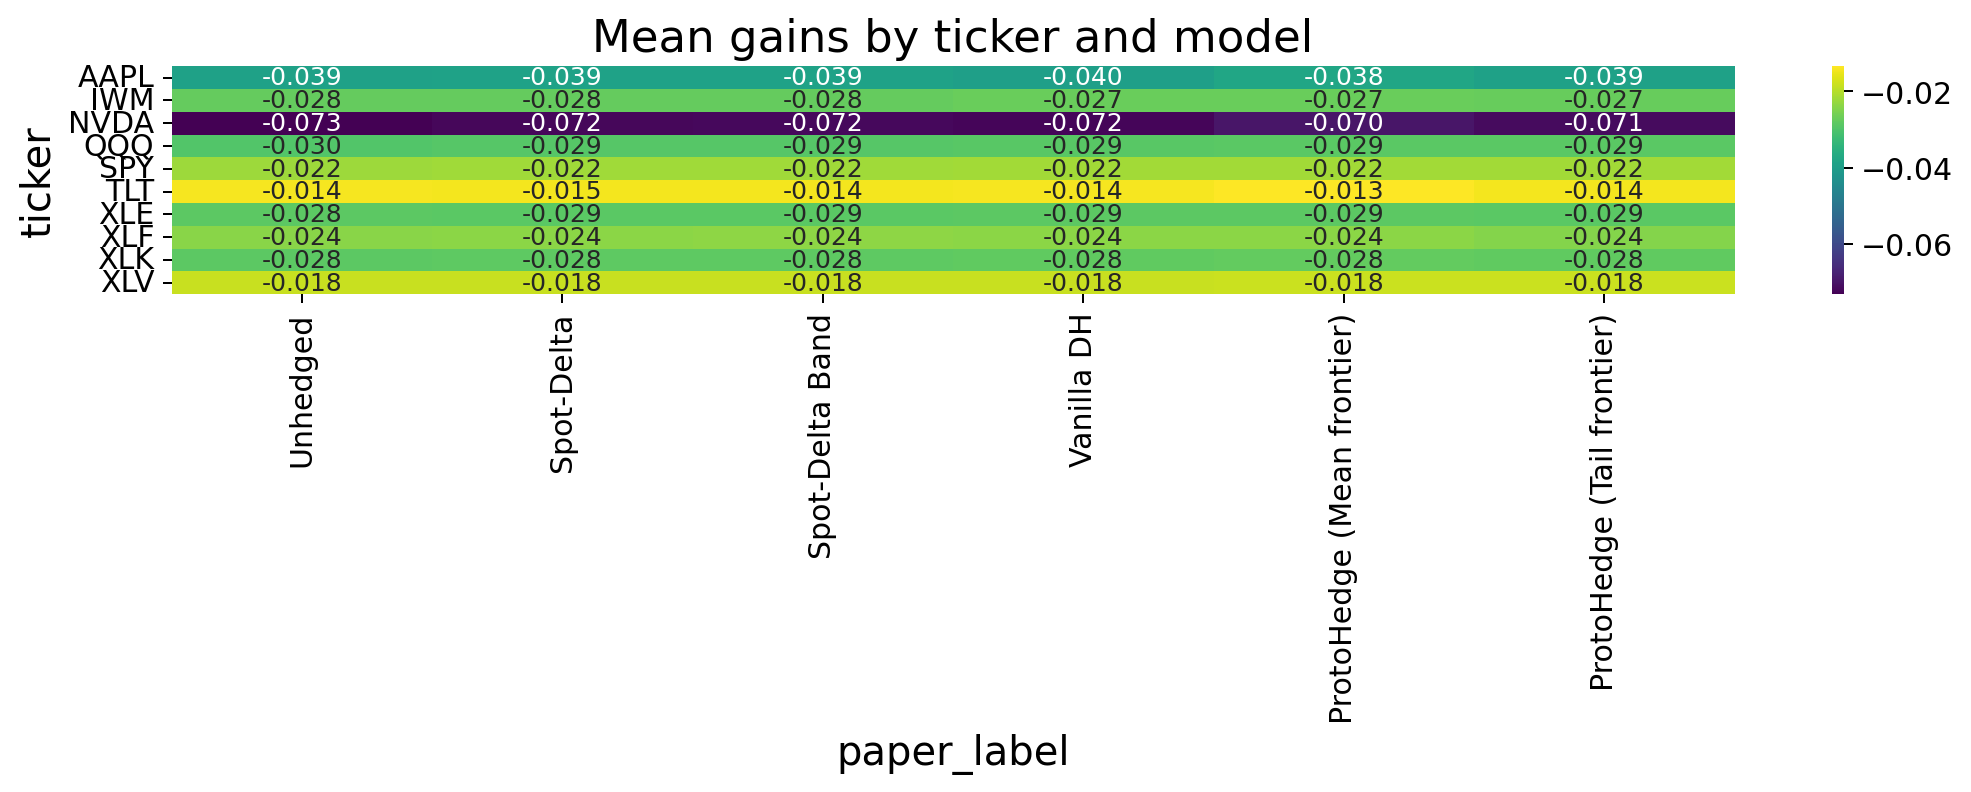
\includegraphics[width=0.9\linewidth]{final_notebook_assets/real_data_panel/panel_mean_heatmap.png}
    \caption{Mean gains across the 10-ticker real-data panel. The mean-oriented ProtoHedge frontier is the strongest average performer and wins on 8 of the 10 tickers.}
    \label{fig:panel-mean-heatmap}
\end{figure}

\begin{figure}[H]
    \centering
    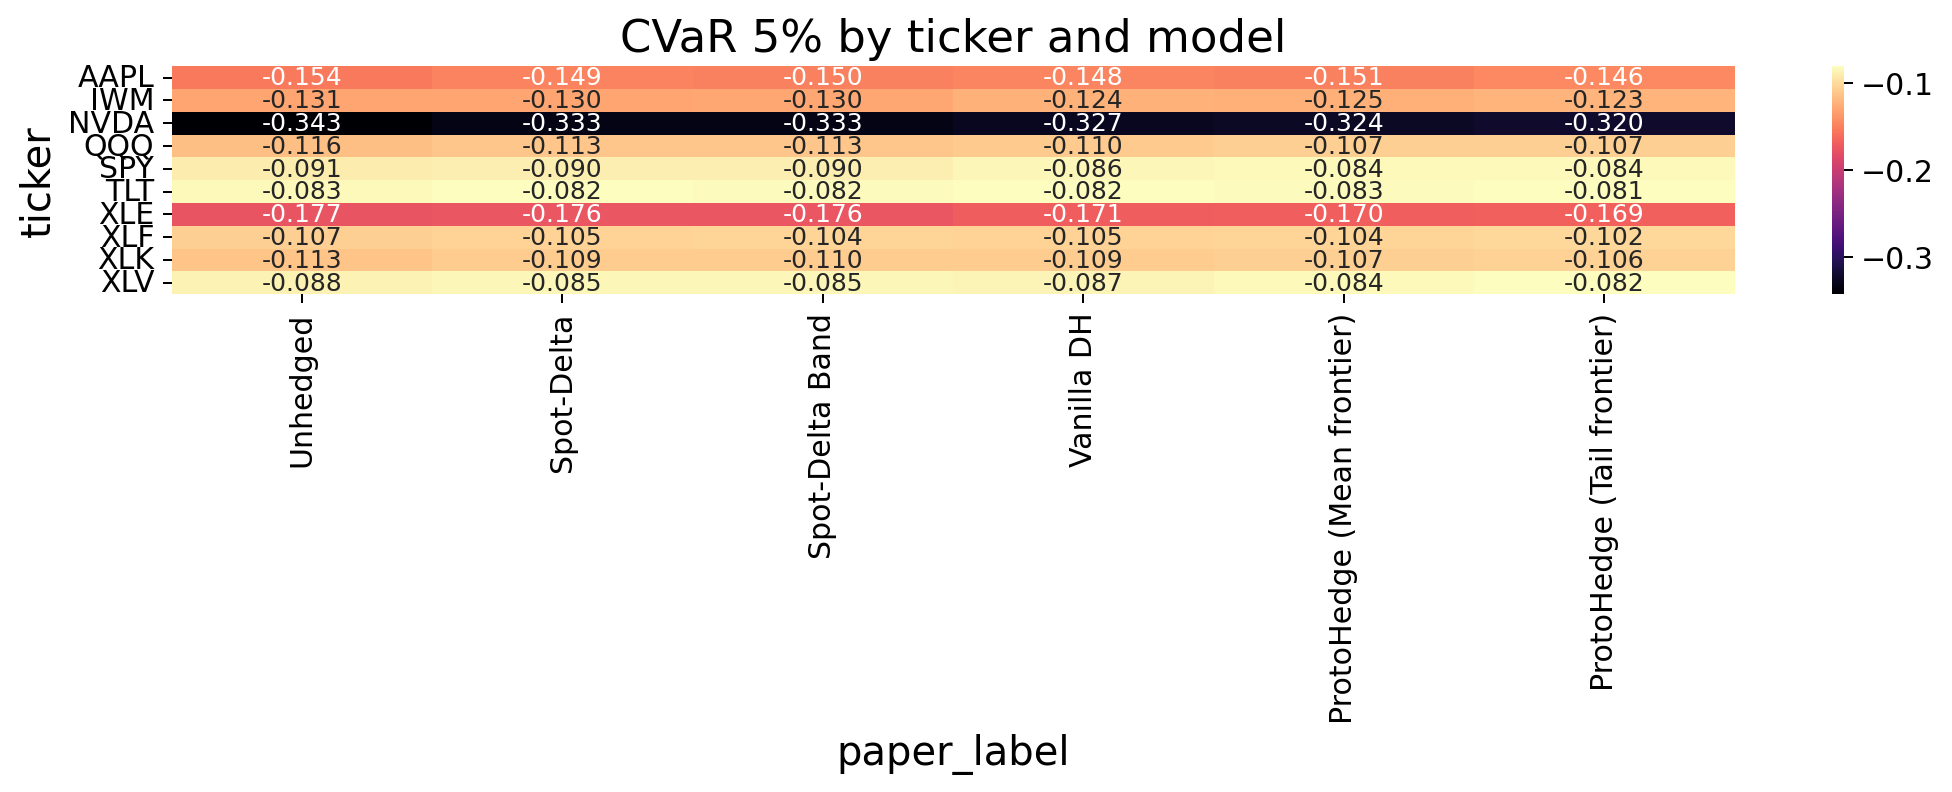
\includegraphics[width=0.9\linewidth]{final_notebook_assets/real_data_panel/panel_cvar_heatmap.png}
    \caption{CVaR$_{5\%}$ across the 10-ticker real-data panel. The tail-oriented ProtoHedge frontier achieves the strongest average tail performance and is the best-CVaR model in 8 of the 10 tickers, while a ProtoHedge model is best on all 10.}
    \label{fig:panel-cvar-heatmap}
\end{figure}

\subsection{Position Bounds and Economic Credibility}
The bound-occupancy diagnostic is central to the empirical interpretation. Vanilla Deep Hedging has average bound occupancy 0.077515, compared with 0.048616 for the ProtoHedge mean frontier and 0.030434 for the ProtoHedge tail frontier. In other words, ProtoHedge is not winning by spending more time on hard position limits than vanilla. On average it is doing the opposite.

This point is important because the single-underlying pilot showed exactly why an unconstrained comparison can be misleading: apparent performance gains can be driven by boundary saturation. The final panel suggests that the performance improvements of the ProtoHedge frontiers are not simply artifacts of more extreme trading.

\begin{figure}[H]
    \centering
    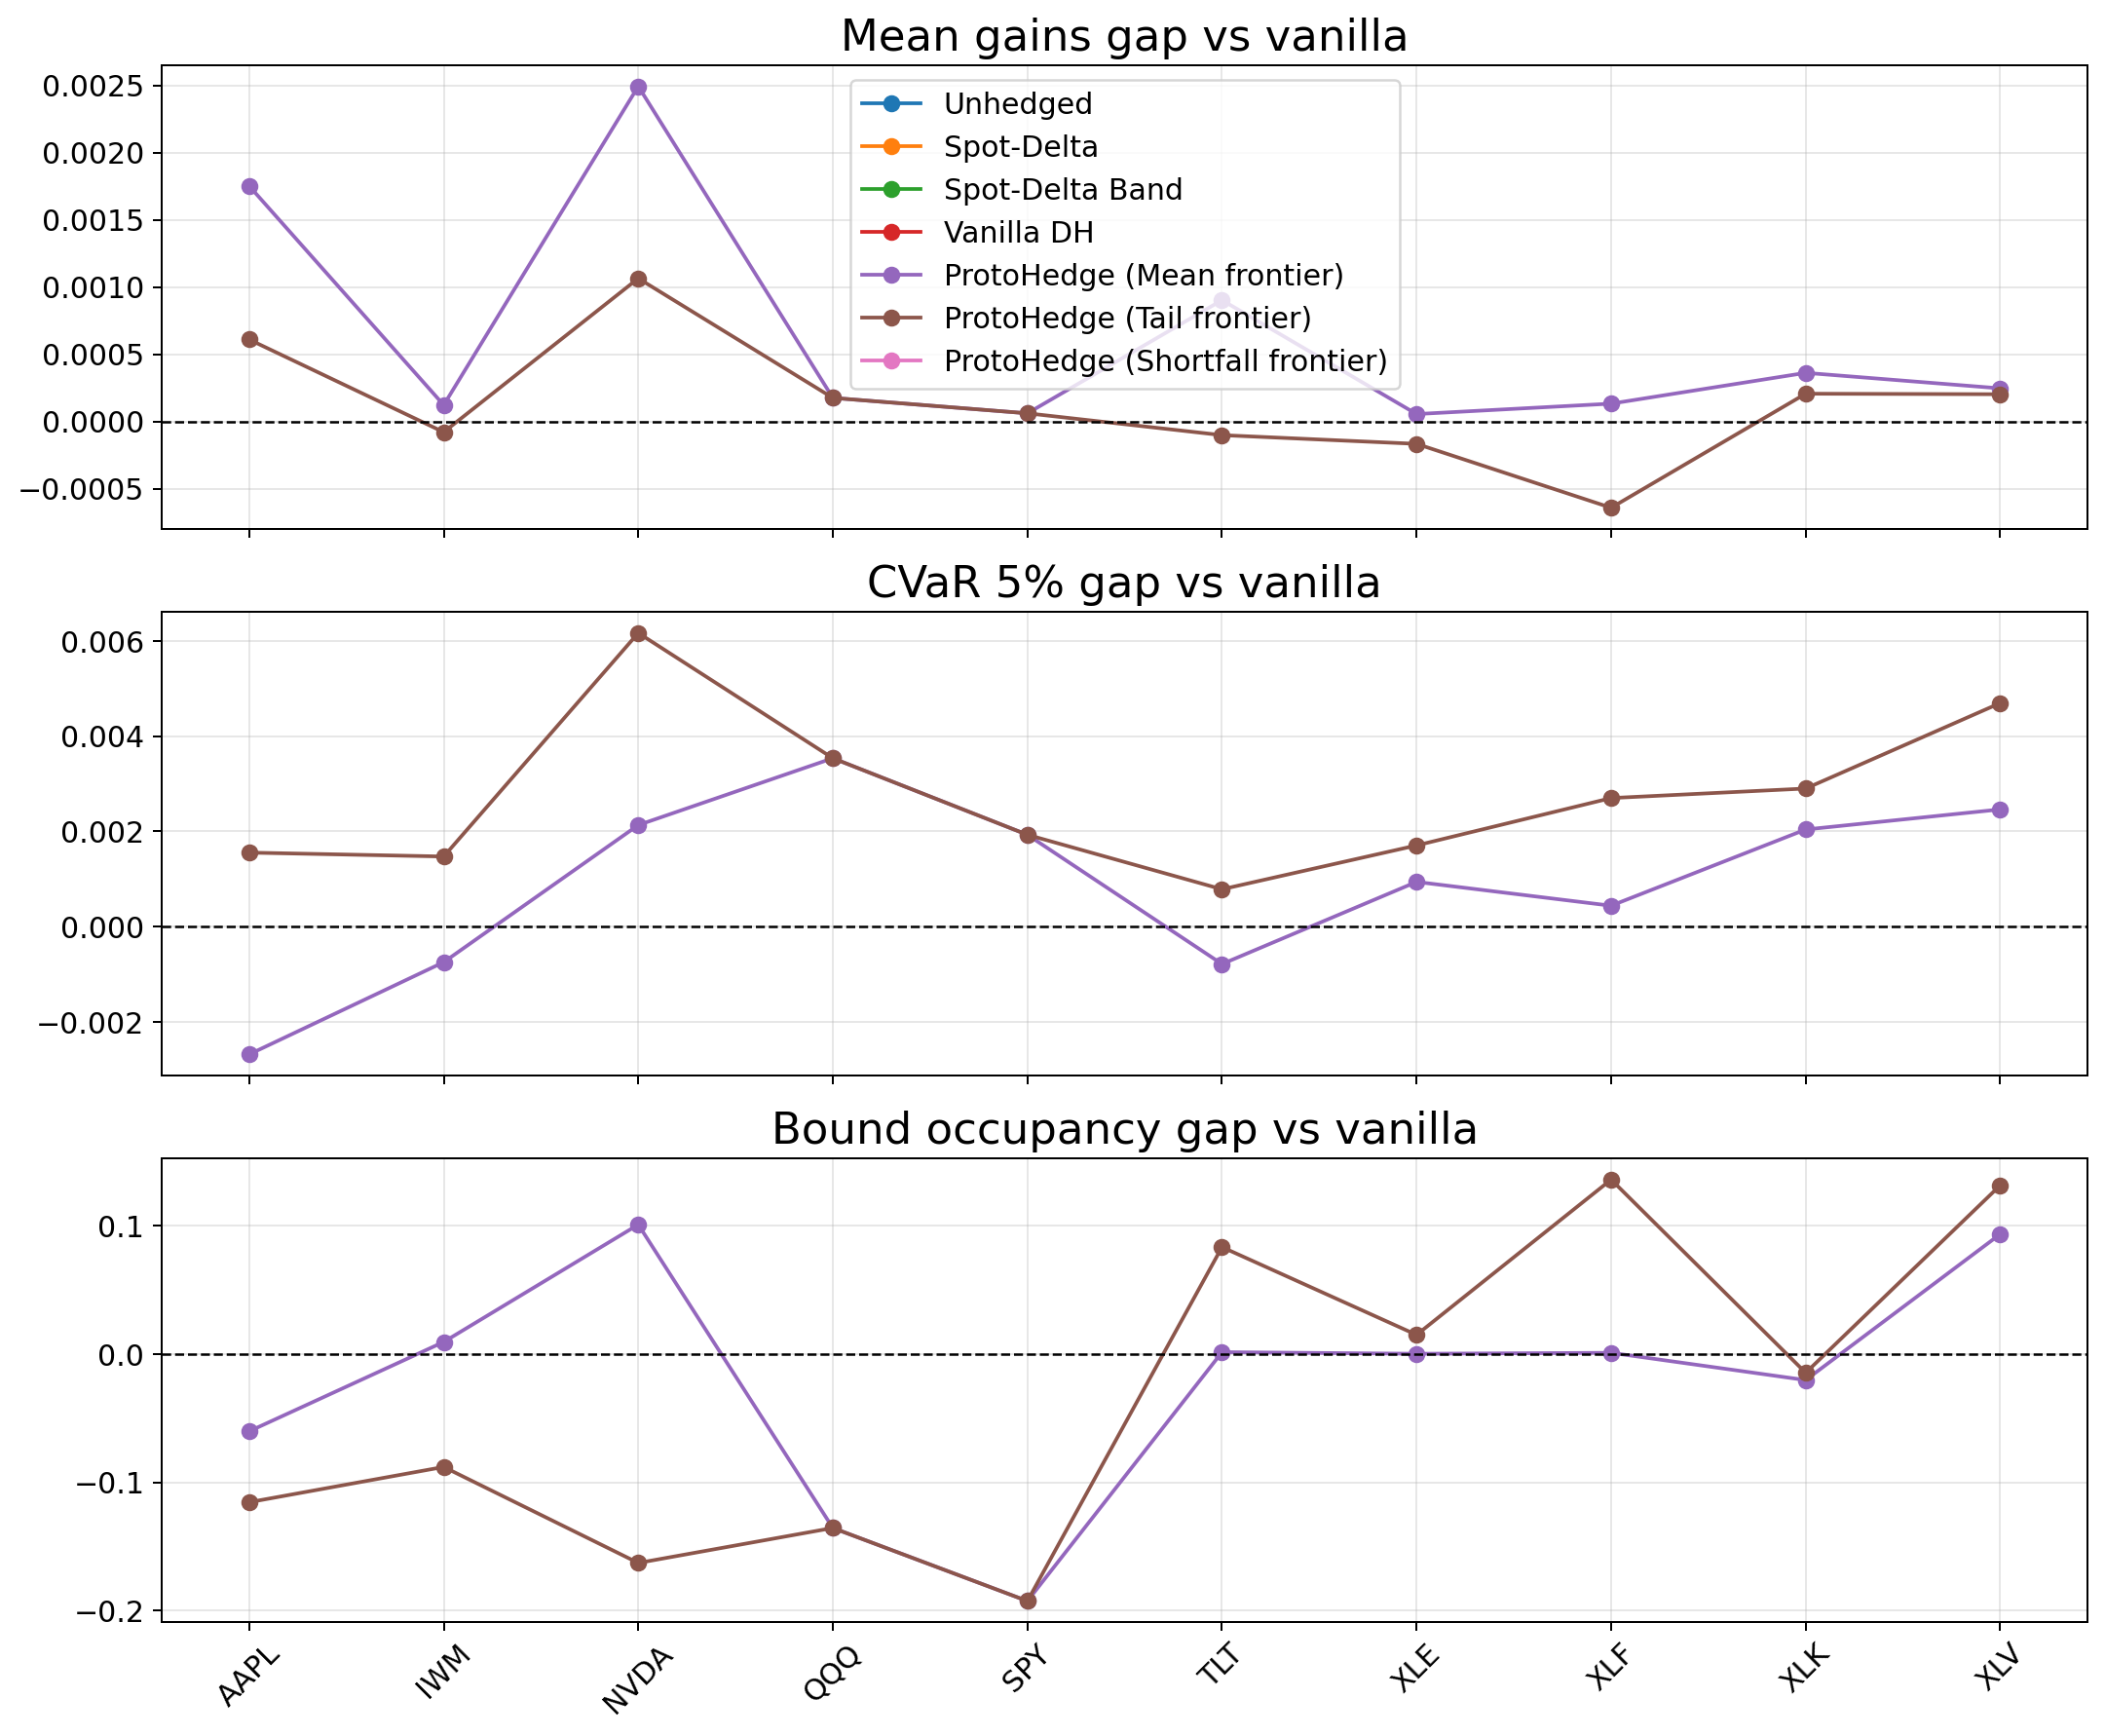
\includegraphics[width=0.9\linewidth]{final_notebook_assets/real_data_panel/panel_proto_vs_vanilla_gaps.png}
    \caption{Per-ticker gaps of the two ProtoHedge frontiers relative to vanilla Deep Hedging. Positive values on the top two panels favor ProtoHedge. Negative values on the bottom panel indicate lower bound occupancy than vanilla.}
    \label{fig:proto-vs-vanilla-gaps}
\end{figure}

\subsection{Rank Stability Across the Panel}
The average-rank summary further strengthens the result. ProtoHedge (Mean frontier) has the best average rank in mean gains (1.2), while ProtoHedge (Tail frontier) has the best average rank in CVaR$_{5\%}$ (1.0). Vanilla Deep Hedging ranks third on mean and third on CVaR among the six reported model labels. The broad picture is therefore stable across multiple ways of summarizing the panel, not just in one chosen metric.

\subsection{Representative Regime Analysis}
To move beyond unconditional averages, we perform a deep-dive regime analysis on QQQ using the selected tail-oriented ProtoHedge artifact. The regime study slices the held-out test set by return, implied-volatility, and drawdown buckets.

The result is not that ProtoHedge dominates in every local regime. Instead, the regime analysis shows state dependence. For example, in the QQQ down-return regime, ProtoHedge improves mean performance and shortfall probability relative to vanilla, but not the 5\% tail itself. In the up-return regime, ProtoHedge improves both mean and CVaR. In mid-volatility and low-volatility episodes, ProtoHedge again improves or matches vanilla on the left tail. This is the pattern one would expect from a model that is genuinely adapting its behavior to market state rather than simply copying a single hedge rule everywhere.

\subsection{Interpretability Verification}
The prototype diagnostics support the interpretability claim directly. For the QQQ deep dive, the top 3 prototypes account for 58.4\% of the total usage mass, and the top 6 account for 82.3\%. By the top 8 prototypes, cumulative usage reaches 94.2\%. The decision rule is therefore concentrated in a small number of recurring states rather than spread diffusely across the full prototype bank.

The dominant prototypes are also regime-sensitive. In QQQ, prototype 21 dominates down-return and high-volatility regimes, while prototype 8 dominates middle and up-return regimes as well as low- and mid-volatility regimes. These regime-dependent usage shifts are consistent with the idea that the model is routing decisions through distinct and economically meaningful market situations.

\begin{figure}[H]
    \centering
    
\includegraphics[width=0.75\linewidth]{final_notebook_assets/real_data_panel/qqq_prototype_concentration.png}
    \caption{Prototype concentration for the QQQ deep dive. The cumulative-usage curve rises quickly, indicating that a small number of prototypes explain most of the model's decisions.}
    \label{fig:qqq-prototype-concentration}
\end{figure}

We also retrieve the nearest historical states for the most-used prototypes. This step matters because a prototype method is only interpretable if its prototypes map back to recognizable real market states rather than drifting into abstract latent artifacts. In the current run, the nearest-state analysis shows that the dominant prototypes correspond to realistic near-the-money states with different option price levels, times to maturity, and hedge adjustments.

\begin{figure}[H]
    \centering
    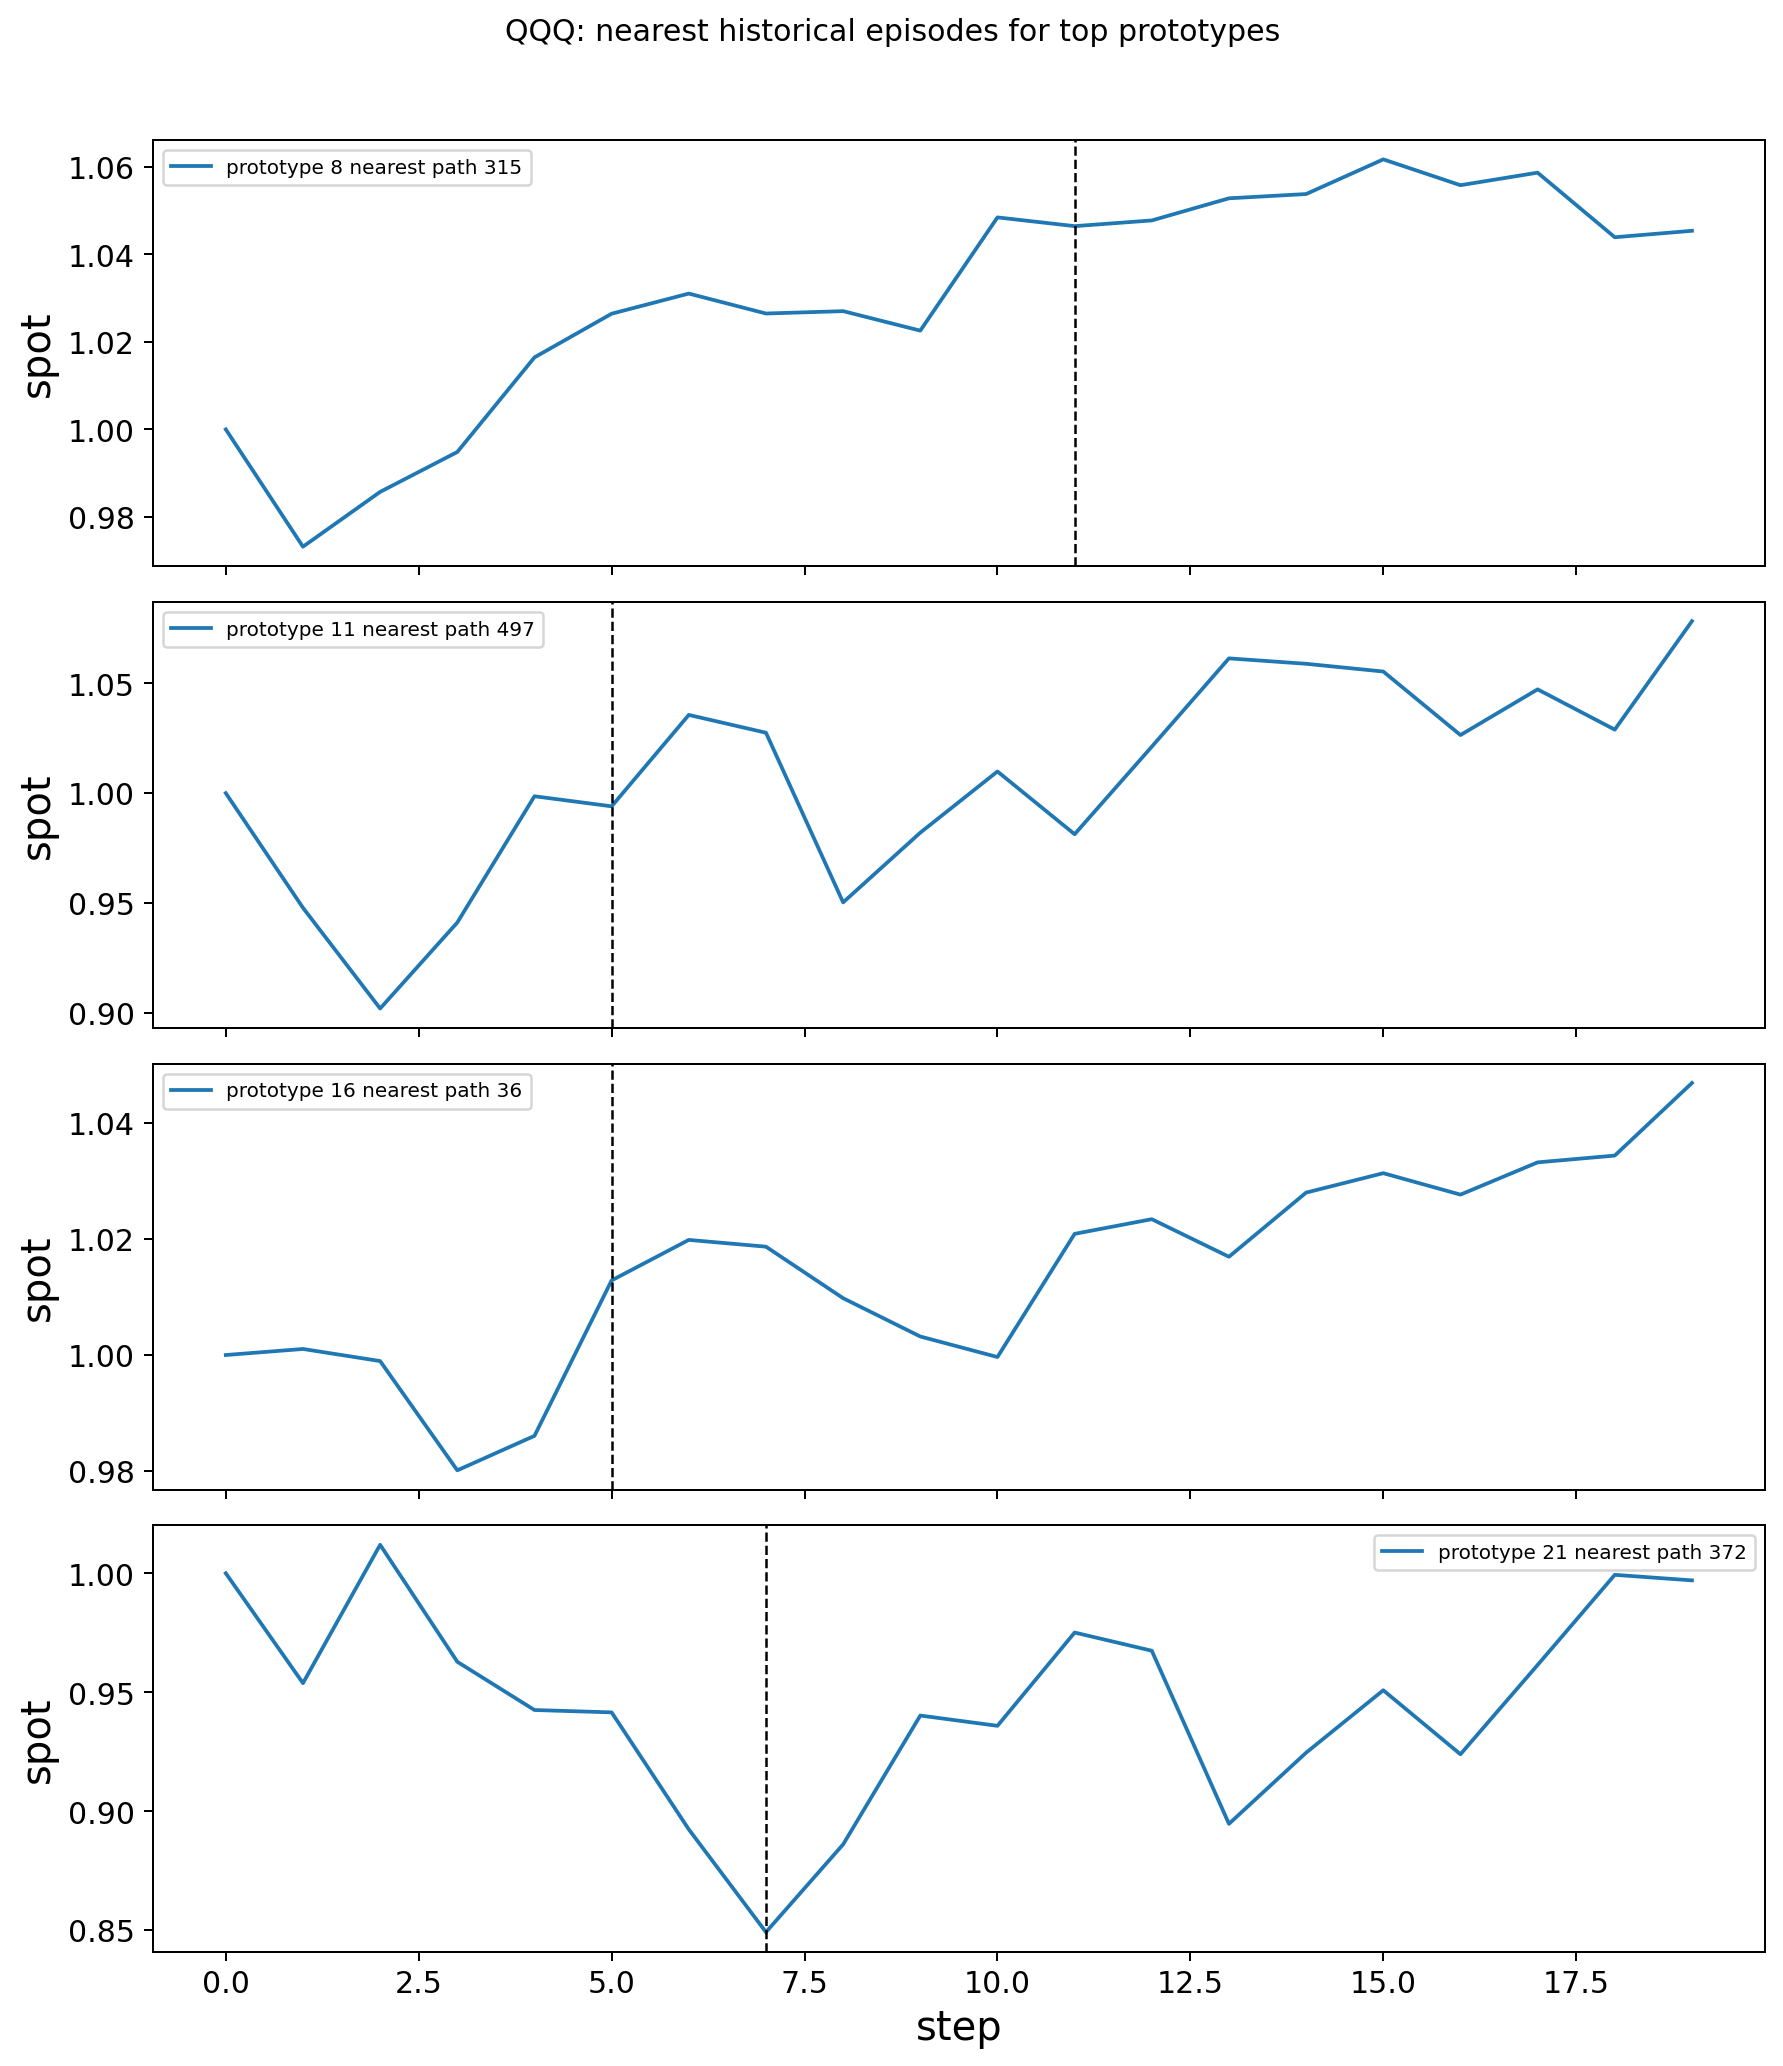
\includegraphics[width=0.9\linewidth]{final_notebook_assets/real_data_panel/qqq_nearest_historical_episodes.png}
    \caption{Nearest historical episodes for the dominant QQQ prototypes. The dashed vertical line marks the time step at which the nearest state is matched to the prototype.}
    \label{fig:qqq-nearest-episodes}
\end{figure}

\subsection{What the Results Support --- and What They Do Not}
The present results support a specific empirical claim: ProtoHedge can preserve, and in many cases slightly improve, the risk--return tradeoff of vanilla Deep Hedging while imposing a more interpretable prototype structure. The results do \emph{not} support a claim of universal dominance, nor do they show that every interpretability metric is solved. The shortfall metric is less clean than mean and CVaR in this panel and should be treated as secondary. Likewise, the strongest interpretability case study currently comes from a representative ticker deep dive rather than from a full multi-ticker prototype analysis.

Still, the central claim survives the main empirical challenge. The advantage of ProtoHedge is no longer limited to synthetic simulation or a single historical panel. It extends to a broad real-data cross section with explicit position-bound controls and direct interpretability checks.

\begin{thebibliography}{9}

\bibitem{buehler2019deephedging}
Hans Buehler, Lukas Gonon, Josef Teichmann, and Ben Wood.
\newblock Deep hedging.
\newblock \emph{Quantitative Finance}, 19(8):1271--1291, 2019.

\bibitem{protohedge2025}
ProtoHedge original paper.
\newblock Placeholder citation to be replaced with the final bibliographic entry from the original manuscript.

\bibitem{wrds}
Wharton Research Data Services (WRDS).
\newblock Placeholder citation for the data source and accessed databases.

\end{thebibliography}

\end{document}
